\chapter{Project File}
\label{chp:intro}

\section{Original Instruction}
A feedback control system for a swinging robotic gymnast must be designed, implemented and verified. Feedback control loops must be designed that use the "legs" of the gymnast to swing the "body" of the gymnast from a "hanging" position to a "handstand" position and then balance the gymnast on top of the horizontal bar. A mathematical model for the dynamics of the swinging robotic gymnast system must be derived or sourced from literature. The dynamics must be analysed to propose an appropriate feedback control architecture that actuates the "legs" of the gymnast using feedback from sensors that measure the swinging motion of the gymnast on a horizontal bar. A practical demonstrator must be constructed and the correct operation must be demonstrated.


\includepdf[pages=1,pagecommand={\section{Project Proposal} \thispagestyle{empty} \label{sec:proposal}}, fitpaper=true]{./figs/proposal/Proposal.pdf}

\includepdf[pages=2-,pagecommand={\thispagestyle{empty}}, fitpaper=true]{./figs/proposal/Proposal.pdf}



\includepdf[pages=1,pagecommand={\section{Progress Report} \thispagestyle{empty} \label{sec:progress_report}}, fitpaper=true]{./figs/progress_report/progress_report.pdf}

\includepdf[pages=2-,pagecommand={\thispagestyle{empty}}, fitpaper=true]{./figs/progress_report/progress_report.pdf}




\includepdf[pages=1,pagecommand={\section{Preliminary Final} \thispagestyle{empty} \label{sec:preliminary_final}}, fitpaper=true]{./figs/draft/prelim_final.pdf}

\includepdf[pages=2-56,pagecommand={\thispagestyle{empty}}, fitpaper=true]{./figs/draft/prelim_final.pdf}

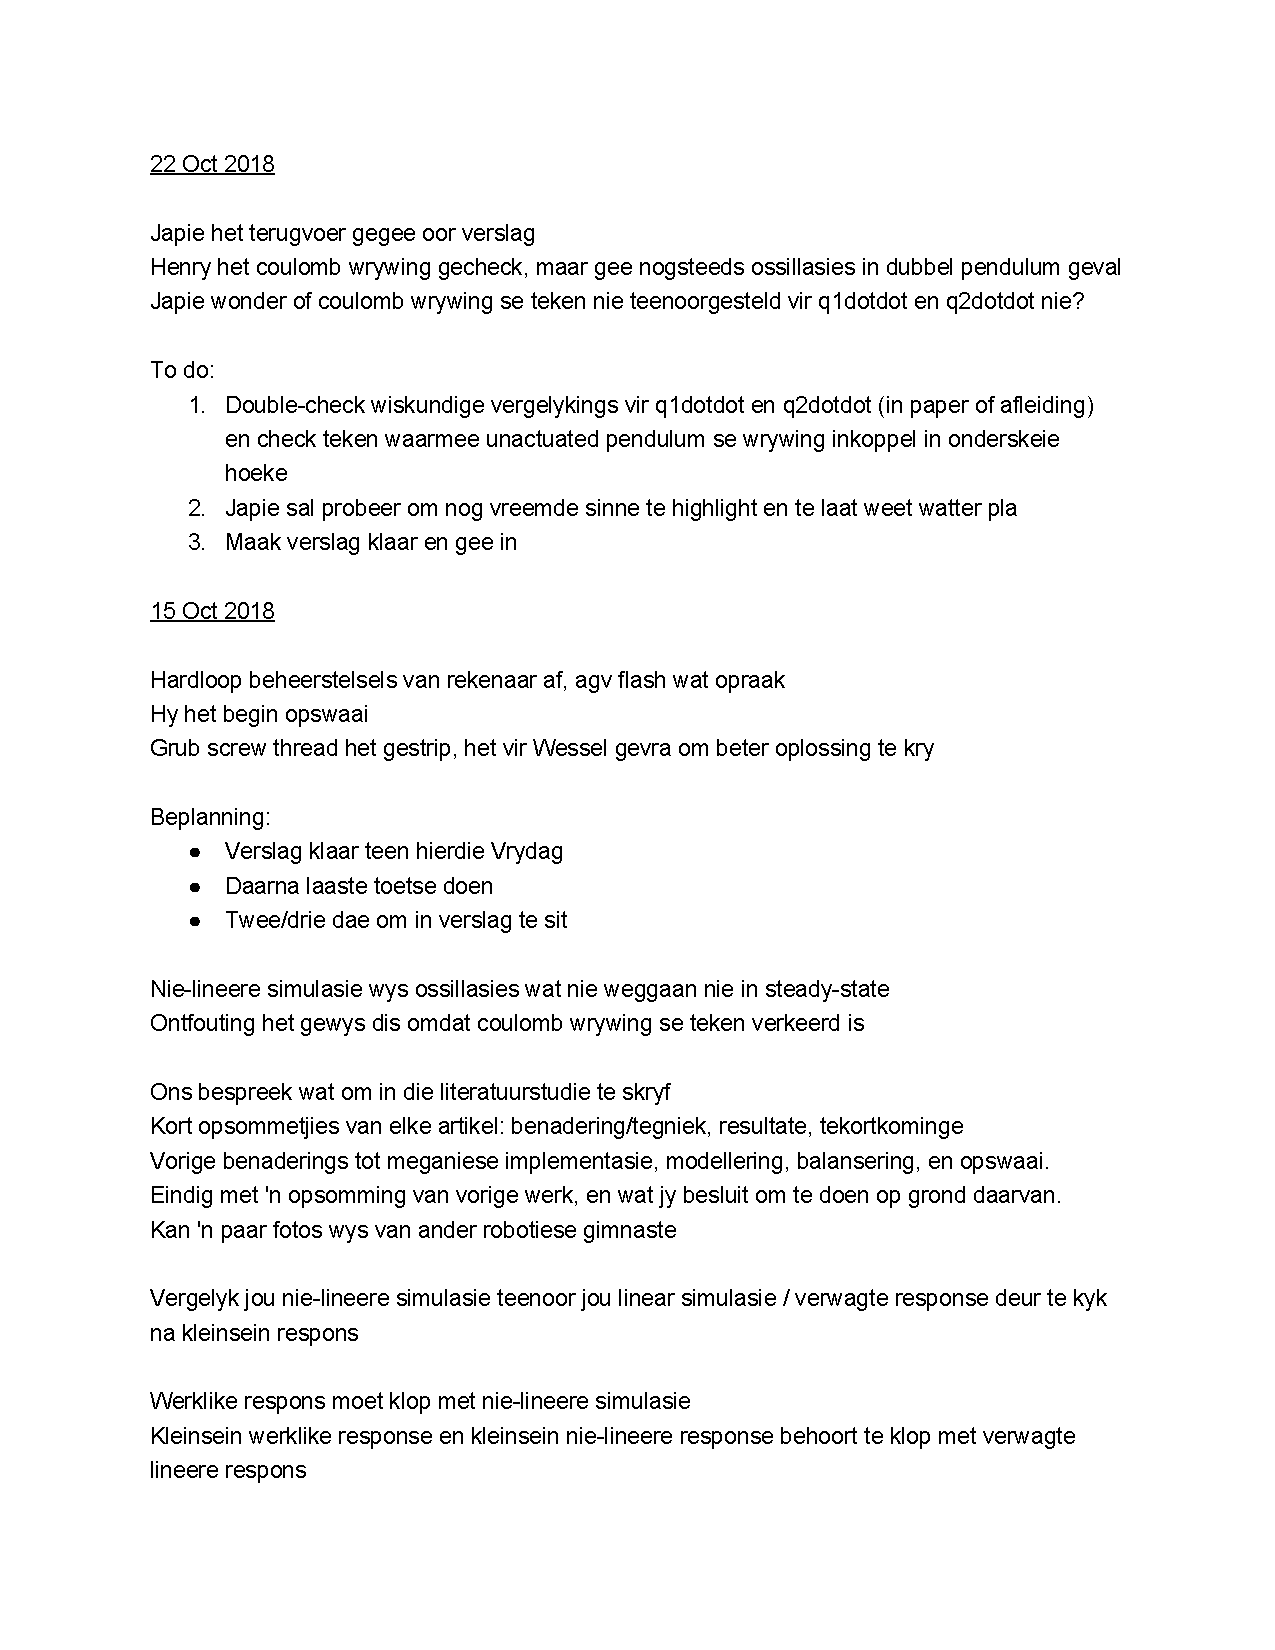
\includepdf[pages=1,pagecommand={\section{Weekly Progress Report} \thispagestyle{empty} \label{sec:weekly}}, fitpaper=true]{./Meeting_Notes.pdf}
\includepdf[pages=2-,pagecommand={\thispagestyle{empty}}, fitpaper=true]{./Meeting_Notes.pdf}








